\chapter{Realizacja projektu}


\section{Wykorzystane technologie}

\subsection{Język programowania Python}

Kod projektu został napisany w języku Python. Wybór tego języka był spowodowany szeroką dostępnością bibliotek i
narzędzi wspomagających uczenie maszynowe. W szczególności należy zwrócić uwagę na biblioteki \textit{PyTorch} (użyta w projekcie) oraz \textit{Tensorflow} (alternatywa).
Są to dwie najpopularniejsze biblioteki do operowania na tensorach (tensor to uogólnienie macierzy na wiele wymiarów).
Obie pozwalają na przyśpieszanie obliczeń z użyciem zewnętrznych akceleratorów takich jak np. karty graficzne.

Podczas prac badawczych, wykorzystana wersja Pythona to \textit{3.12.0}.

\subsection{Biblioteka PyTorch}

Biblioteka PyTorch jest obecnie najpopularniejszą biblioteką uczenia maszynowego.
Pozwala ona projektować obliczenia w formie modułów i posiada silnik automatycznego różniczkowania grafu obliczeniowego (z ang. \textit{autograd}).
Owy silnik jest kluczowy z perspektywy trenowania sieci neuronowych, ponieważ jest w stanie optymalizować parametry modelu.
Warto zwrócić uwagę na to, że PyTorch stawia nacisk na przejrzystość obliczeń - dla porównania operacje w Tensorflow są nierzadko
ukryte pod gotowymi funkcjami (zob. listing~\ref{lst:tensorflow_sample} i~\ref{lst:pytorch_sample})

\begin{lstlisting}[language=ipython,caption={Przykładowa sieć neuronowa w Tensorflow},label={lst:tensorflow_sample}]
tensorflow_model = tf.keras.Sequential([
    tf.keras.layers.Flatten(input_shape=(28, 28)),
    tf.keras.layers.Dense(128, activation='relu'),
    tf.keras.layers.Dense(10, activation='softmax')
])

tensorflow_model.compile() # Brak doglebnej kontroli nad przeplywem obliczen
\end{lstlisting}


\begin{lstlisting}[language=ipython,caption={Przykładowa sieć neuronowa w PyTorch},label={lst:pytorch_sample}]
class PyTorchNetwork(nn.Module):
    def __init__(self):
        super(Net, self).__init__()
        self.flatten = nn.Flatten()
        self.fc1 = nn.Linear(28 * 28, 128)
        self.relu = nn.ReLU()
        self.fc2 = nn.Linear(128, 10)

    def forward(self, x): # Dokladna kontrola nad przeplywem obliczen
        x = self.flatten(x)
        x = self.fc1(x)
        x = self.relu(x)
        x = self.fc2(x)
        return x
\end{lstlisting}

PyTorch oferuje również zestaw narzędzi do przetwarzania danych, dostarcza również gotowe, pretrenowane modele dla najpopularniejszych architektur.
Przykładami są pakiety \textit{torchvision} lub \textit{torch.utils}. Biblioteka jest w stanie wykorzystywać karty graficzne (z ang. \textit{graphical processing unit, GPU}) do przyspieszania obliczeń.

\subsection{Biblioteka OpenCV}

Biblioteka OpenCV \cite{opencv} dostarcza implementacje wielu algorytmów wizji komputerowej.
OpenCV \textcolor{red}{zawiera} interfejs programistyczny, dzięki któremu programista Pythona może komunikować się z implementacją algorytmów w C++.
To zapewnia szybkość wykonywania obliczeń, jednocześnie nie wymuszając na programiście pisania kodu w C++. Przykład wykorzystania biblioteki OpenCV widoczny jest na listingu \ref{lst:opencv_sample}
- kod wylicza momenty Hu.

OpenCV w niniejszym projekcie jest wykorzystywane do automatycznej ekstrakcji obrazów z komórkami na podstawie dużego zdjęcia spod mikroskopu.
Więcej informacji na ten temat znajduje się w rozdziale \ref{sec:kwadraty}.

\begin{lstlisting}[language=ipython,caption={Obliczenie momentów Hu z użyciem OpenCV}, label={lst:opencv_sample}]
import cv2

image = cv2.imread('obraz.jpg', 0)  # 0 oznacza wczytanie obrazu w odcieniach szarosci

hu_moments = cv2.HuMoments(cv2.moments(image)).flatten()

print("Momenty Hu:")
for i in range(0, 7):
    print(f"Moment {i+1}: {hu_moments[i]}")
\end{lstlisting}

\subsection{Inne narzędzia}

Kod źródłowy projektu jest przechowywany w repozytorium na platformie GitHub (dostępny pod adresem \url{https://github.com/matisiekpl/thesis}).
Wykresy były generowane za pomocą biblioteki \textit{matplotlib} \cite{matplotlib},
a metryki liczone z użyciem funkcji pakietu \textit{scikit-learn} \cite{scikit_learn}.

\subsection{Sprzęt}

Do prac badawczych został użyty Apple Macbook Pro 2020 (M1/16GB pamięci).
Trenowanie sieci odbywało się na platformie \textit{kaggle.com}, która oferuje bezpłatne 30 godzin obliczeń co miesiąc z kartą graficzną \textit{NVIDIA P100}.


\section{Zbiór danych}

Wykorzystany w projekcie zbiór danych to kolekcja 170 tysięcy zdjęć komórek z rozmazów szpiku kostnego.
Zdjęcia mają nadane etykiety przez diagnostów i przedstawiają różne komórki widziane pod mikroskopem.
Próbki szpiku kostnego pochodzą z biopsji 945 pacjentów z Monachijskiego Labolatorium Białaczek (\textit{MLL Münchner Leukämielabor} \cite{mll}).
Akwizycja obrazu polegała na wykonaniu zdjęcia mikroskopią Brightfield'a~\cite{microscopy} z 40-krotnym powiększeniem.
Producentem mikroskopu było przedsiębiorstwo Fraunhofer IIS.

\begin{figure}
    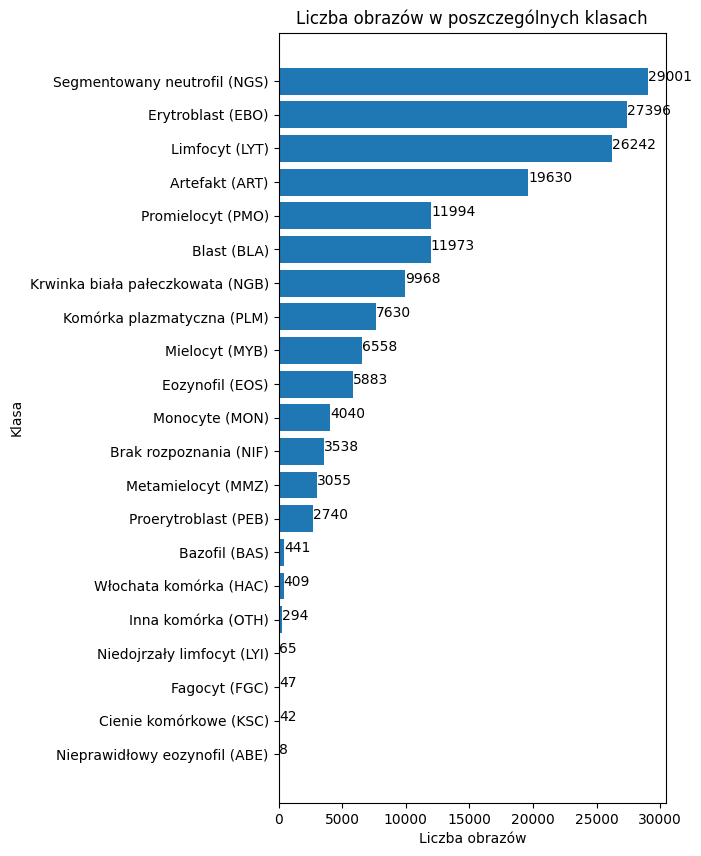
\includegraphics[width=\textwidth]{images_count}
    \caption{Histogram rozkładu próbek w klasach w zbiorze danych}
    \label{fig:images_count_vis}
\end{figure}

\begin{figure}
    \centering
    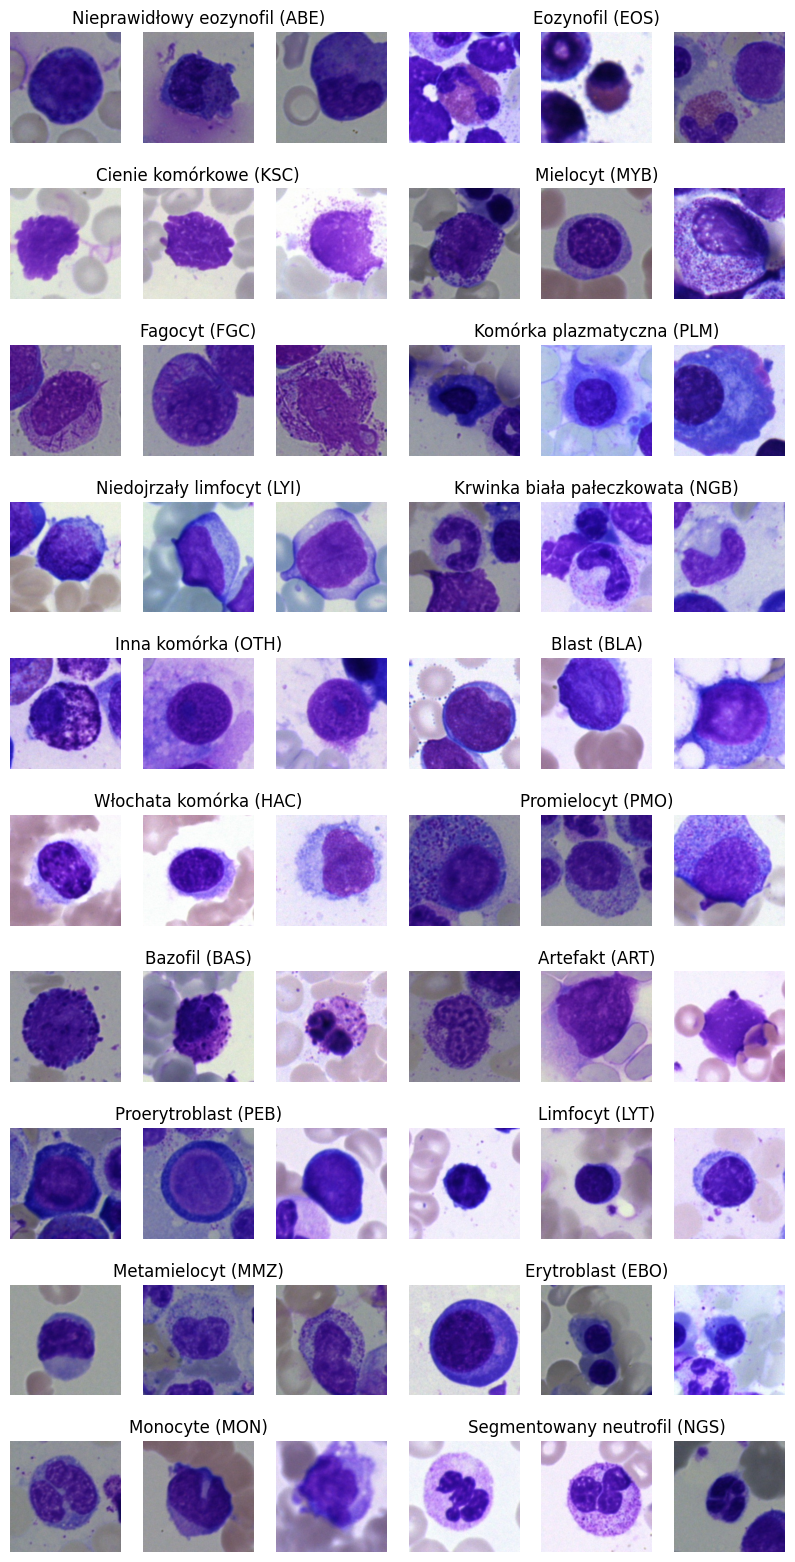
\includegraphics[height=0.9\textheight]{images_examples}
    \caption{Przykładowe zdjęcia komórek ze zbioru danych dla każdej z klas}
    \label{fig:images_examples}
\end{figure}

Komórki były barwione metodą Maya-Grünwalda-Giemsa \cite{histology}.
Zbiór danych zawiera 21 klas, lecz w trakcie trenowania sieci neuronowych wykorzystano jedynie 11 (odrzucone klasy posiadały bardzo małą ilość próbek).
Histogram rozkładu klas jest widoczny na rys. \ref{fig:images_count_vis}.
Zbiór danych jest niezrównoważony, ponieważ ilość obrazów w każdej klasie znacząco się różni.
Przykładowe zdjęcia są widoczne na rys \ref{fig:images_examples}.


\section{Struktura projektu}

\subsection{Przygotowanie danych}

Zbiór danych to katalog ze zdjęciami.
Zdjęcia są pogrupowane w podkatalogach, gdzie jego nazwa oznacza typ komórki.
Każdy podkatalog zawiera kolorowe zdjęcia w formacie \textit{.jpg} w rozmiarze \textit{250 pikseli x 250 pikseli}.
Przed treningiem sieci neuronowej konieczne jest przetwarzanie wstępne zbioru danych (z ang. \textit{preprocessing}).

\begin{lstlisting}[language=ipython,caption={Transformacja danych}, label={lst:transforms}]
transform = transforms.Compose([
    transforms.Resize((224, 224)), # przeskaluj obrazy
    transforms.RandomEqualize(1), # wyrownaj histogram z prawdopodobienstwem 1, czyli dla kazdego obrazu
    transforms.ToTensor(), # zamien na Tensor
    transforms.Normalize(mean=[0.485, 0.456, 0.406], std=[
        0.229, 0.224, 0.225]), # normalizuj wedlug mediany i odch. stand.
])
\end{lstlisting}

Do realizacji przygotowania danych wykorzystano pakiet \textit{torchvision.transforms}.
Kod transformacji jest przedstawiony na listingu~\ref{lst:transforms}.
Wykonuje on przeskalowanie obrazu wejściowego do rozmiaru \textit{224 piksele na 224 piksele}.
Następnie wyrównuje histogram i normalizuje według średniej i odchylenia standardowego (rys.~\ref{fig:transformations_example}).

Wyrównanie histogramu jest konieczne z powodu różnic w odcieniach barwienia Maya-Grünwalda-Giemsa~\cite{stain}.
Przy każdym wykonaniu rozmazu intensywność kolorów komórek jest inna.
Taka normalizacja zapobiega błędnemu nauczeniu się sieci neuronowej ze względu na odcień, a nie kształt i wygląd komórek.

\begin{figure}
    \centering
    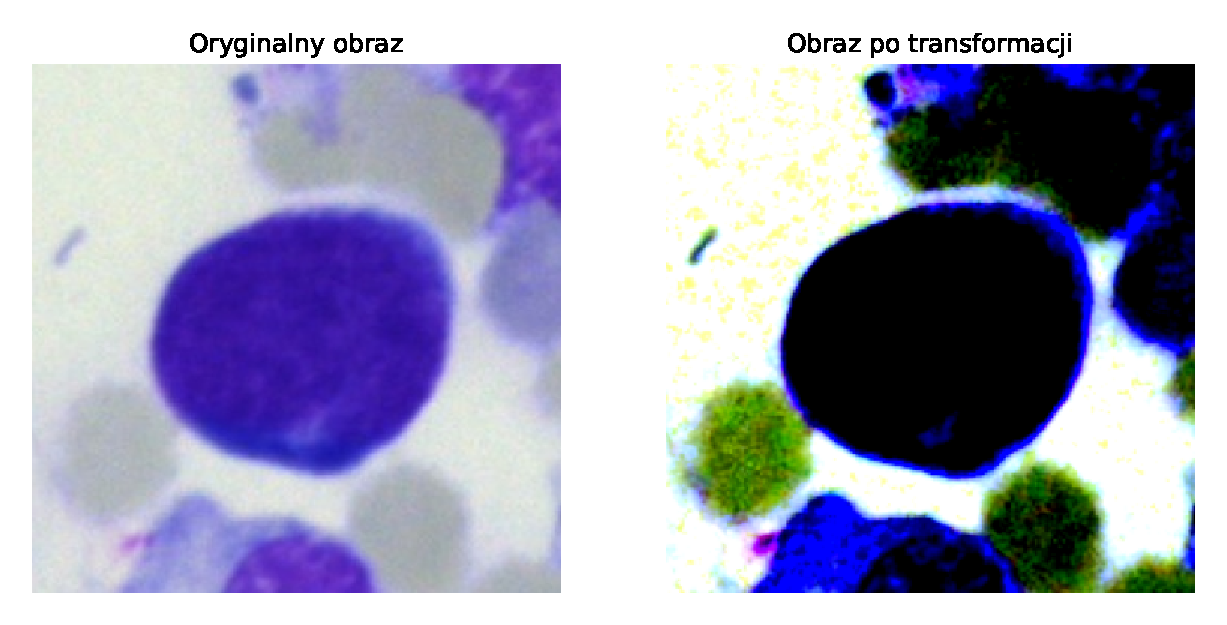
\includegraphics[width=\textwidth]{image_transform}
    \caption{Porównanie obrazu wejściowego przed i po transformacji}
    \label{fig:transformations_example}
\end{figure}

Po przetwarzaniu zbiór danych został podzielony losowo na zestaw treningowy i walidacyjny w proporcjach odpowiednio \textit{80:20}.
Zestaw treningowy służy do optymalizacji parametrów sieci neuronowej.
Zestaw walidacyjny natomiast jest używany do sprawdzania jakości modelu na obrazach, których sieć neuronowa "nigdy nie widziała".

\subsection{Trening sieci neuronowej}

Niniejsza praca ma za zadanie między innymi porównać różne architektury splotowych sieci neuronowych i ocenić,
która z nich wypada najlepiej w zadaniu klasyfikacji komórek z rozmazów szpiku kostnego.
Omówiony poniżej trening sieci neuronowej o architekturze \textit{EfficientNet B0} wygląda tak samo dla innych architektur, takich jak \textit{EfficientNet B5}, \textit{ResNet} i innych.
Współczynnik uczenia wynosił \textit{0.001}, a ilość epok była równa 3.
\textcolor{red}{Niestety z powodu ograniczeń infrastruktury do trenowania, nie udało się wykonać walidacji krzyżowej dla każdego z modeli osobno. Zbiór walidacyjny był natomiast wybierany losowo za każdym razem, gdy badano nową sieć neuronową.}

Trenowanie sieci neuronowej z użyciem biblioteki PyTorch sprowadza się do iterowania po zbiorze wejściowym i wykonywania kroku optymalizacyjnego przy każdym przejściu.
Uproszczony schemat działania głównej pętli treningowej (kod przestawiony na listingu~\ref{lst:train}):

\begin{enumerate}
    \item Pobranie miniwsadu z próbkami treningowymi i skopiowanie ich na urządzenie zewnętrzne, czyli kartę graficzną.
    \item Wykonanie przejścia w przód sieci neuronowej.
    Oznacza to obliczenie wartości neuron na warstwie wyjściowej na bazie uprzednio pobranych próbek.
    \item Porównanie wyjścia sieci neuronowej z oczekiwanymi predykcjami i obliczenie błędu sieci.
    \item Obliczenie gradientów za pomocą algorytmu propagacji wstecznej.
    \item Wykonanie kroku optymalizacyjnego z użyciem optymalizatora \textit{Adam}.
    \item Obliczenie metryk dla zbioru walidacyjnego i zapisanie ich.
\end{enumerate}

\lstinputlisting[label={lst:train}, caption={Kod pętli treningowej w języku Python z wykorzystaniem PyTorch}, language=ipython]{train.py}

\subsection{Ewaluacja jakości modelu}

\begin{figure}
    \centering
    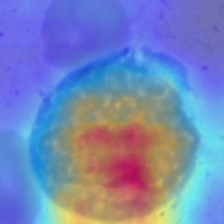
\includegraphics[width=0.5\textwidth]{cam}
    \caption{Mapa cieplna GradCAM dla obrazu komórki plazmatycznej}
    \label{fig:cam}
\end{figure}

\textcolor{red}{
    Wyjściem modelu jest rozkład prawdopodobieństwa rozpoznania poszczególnych rodzajów komórek oraz mapa cieplna GradCAM.
    Przykładowa mapa cieplna jest widoczna na rys.~\ref{fig:cam}.
    Przedstawia ona miejsca na obrazie, które najbardziej wpłynęły na predykcję.
}

Do sprawdzenia jakości modelu uczenia maszynowego konieczny jest dobór właściwych metryk.
Ze względu na to, że trenowany jest klasyfikator wieloklasowy, a zbiór danych nie jest zrównoważony, zwykłe metryki takie jak dokładność (z ang. \textit{accuracy}) nie wystarczą.
Dla każdej klasy jest liczona precyzja (z ang. \textit{precision}) i czułość (z ang. \textit{recall}).
Obie te metryki składają się do obliczenia wyniku F1 (z ang. \textit{F1-score})~\cite{geron}.
Co ważne, wynik F1 jest liczony z uwzględnieniem wag poszczególnych klas.
Obliczana jest również macierz pomyłek.
Informuje ona o tym, które klasy są najczęściej mylone między sobą.
Metryki są zapisywane do pliku tekstowego oraz do plików obrazów w celu późniejszej analizy.


\section{Interfejs użytkownika}

W celu łatwego korzystania z modelu uczenia maszynowego przez diagnostów \textcolor{red}{opracowana została} aplikacja internetowa do interakcji z nim.
Zrzut ekranu interfejsu użytkownika jest widoczny na rys.~\ref{fig:ui}.
Aplikacja została napisana z użyciem \textit{Vue}~\cite{vue} - biblioteki do tworzenia interaktywnych interfejsów użytkownika dla sieci web.
Łączy się ona z serwerem HTTP napisanym z użyciem biblioteki Flask~\cite{flask}.
Serwer eksponuje interfejs REST API, który dla wysłanego zdjęcia zwraca rozkład prawdopodobieństwa \textcolor{red}{ rozpoznania poszczególnych klas}.
Przed wywołaniem modelu, funkcja upewnia się, że przychodzący obrazek jest poprawnego formatu.
Dopiero po zwalidowaniu poprawności danych, kod przystępuje do utworzenia rozkładu prawdopodobieństwa (zmienna \textit{result}).
Renderowana jest również mapa cieplna GradCAM informująca użytkownika o regionach obrazu, które były kluczowe dla modelu w trakcie wykonywania predykcji.


\begin{figure}
    \centering
    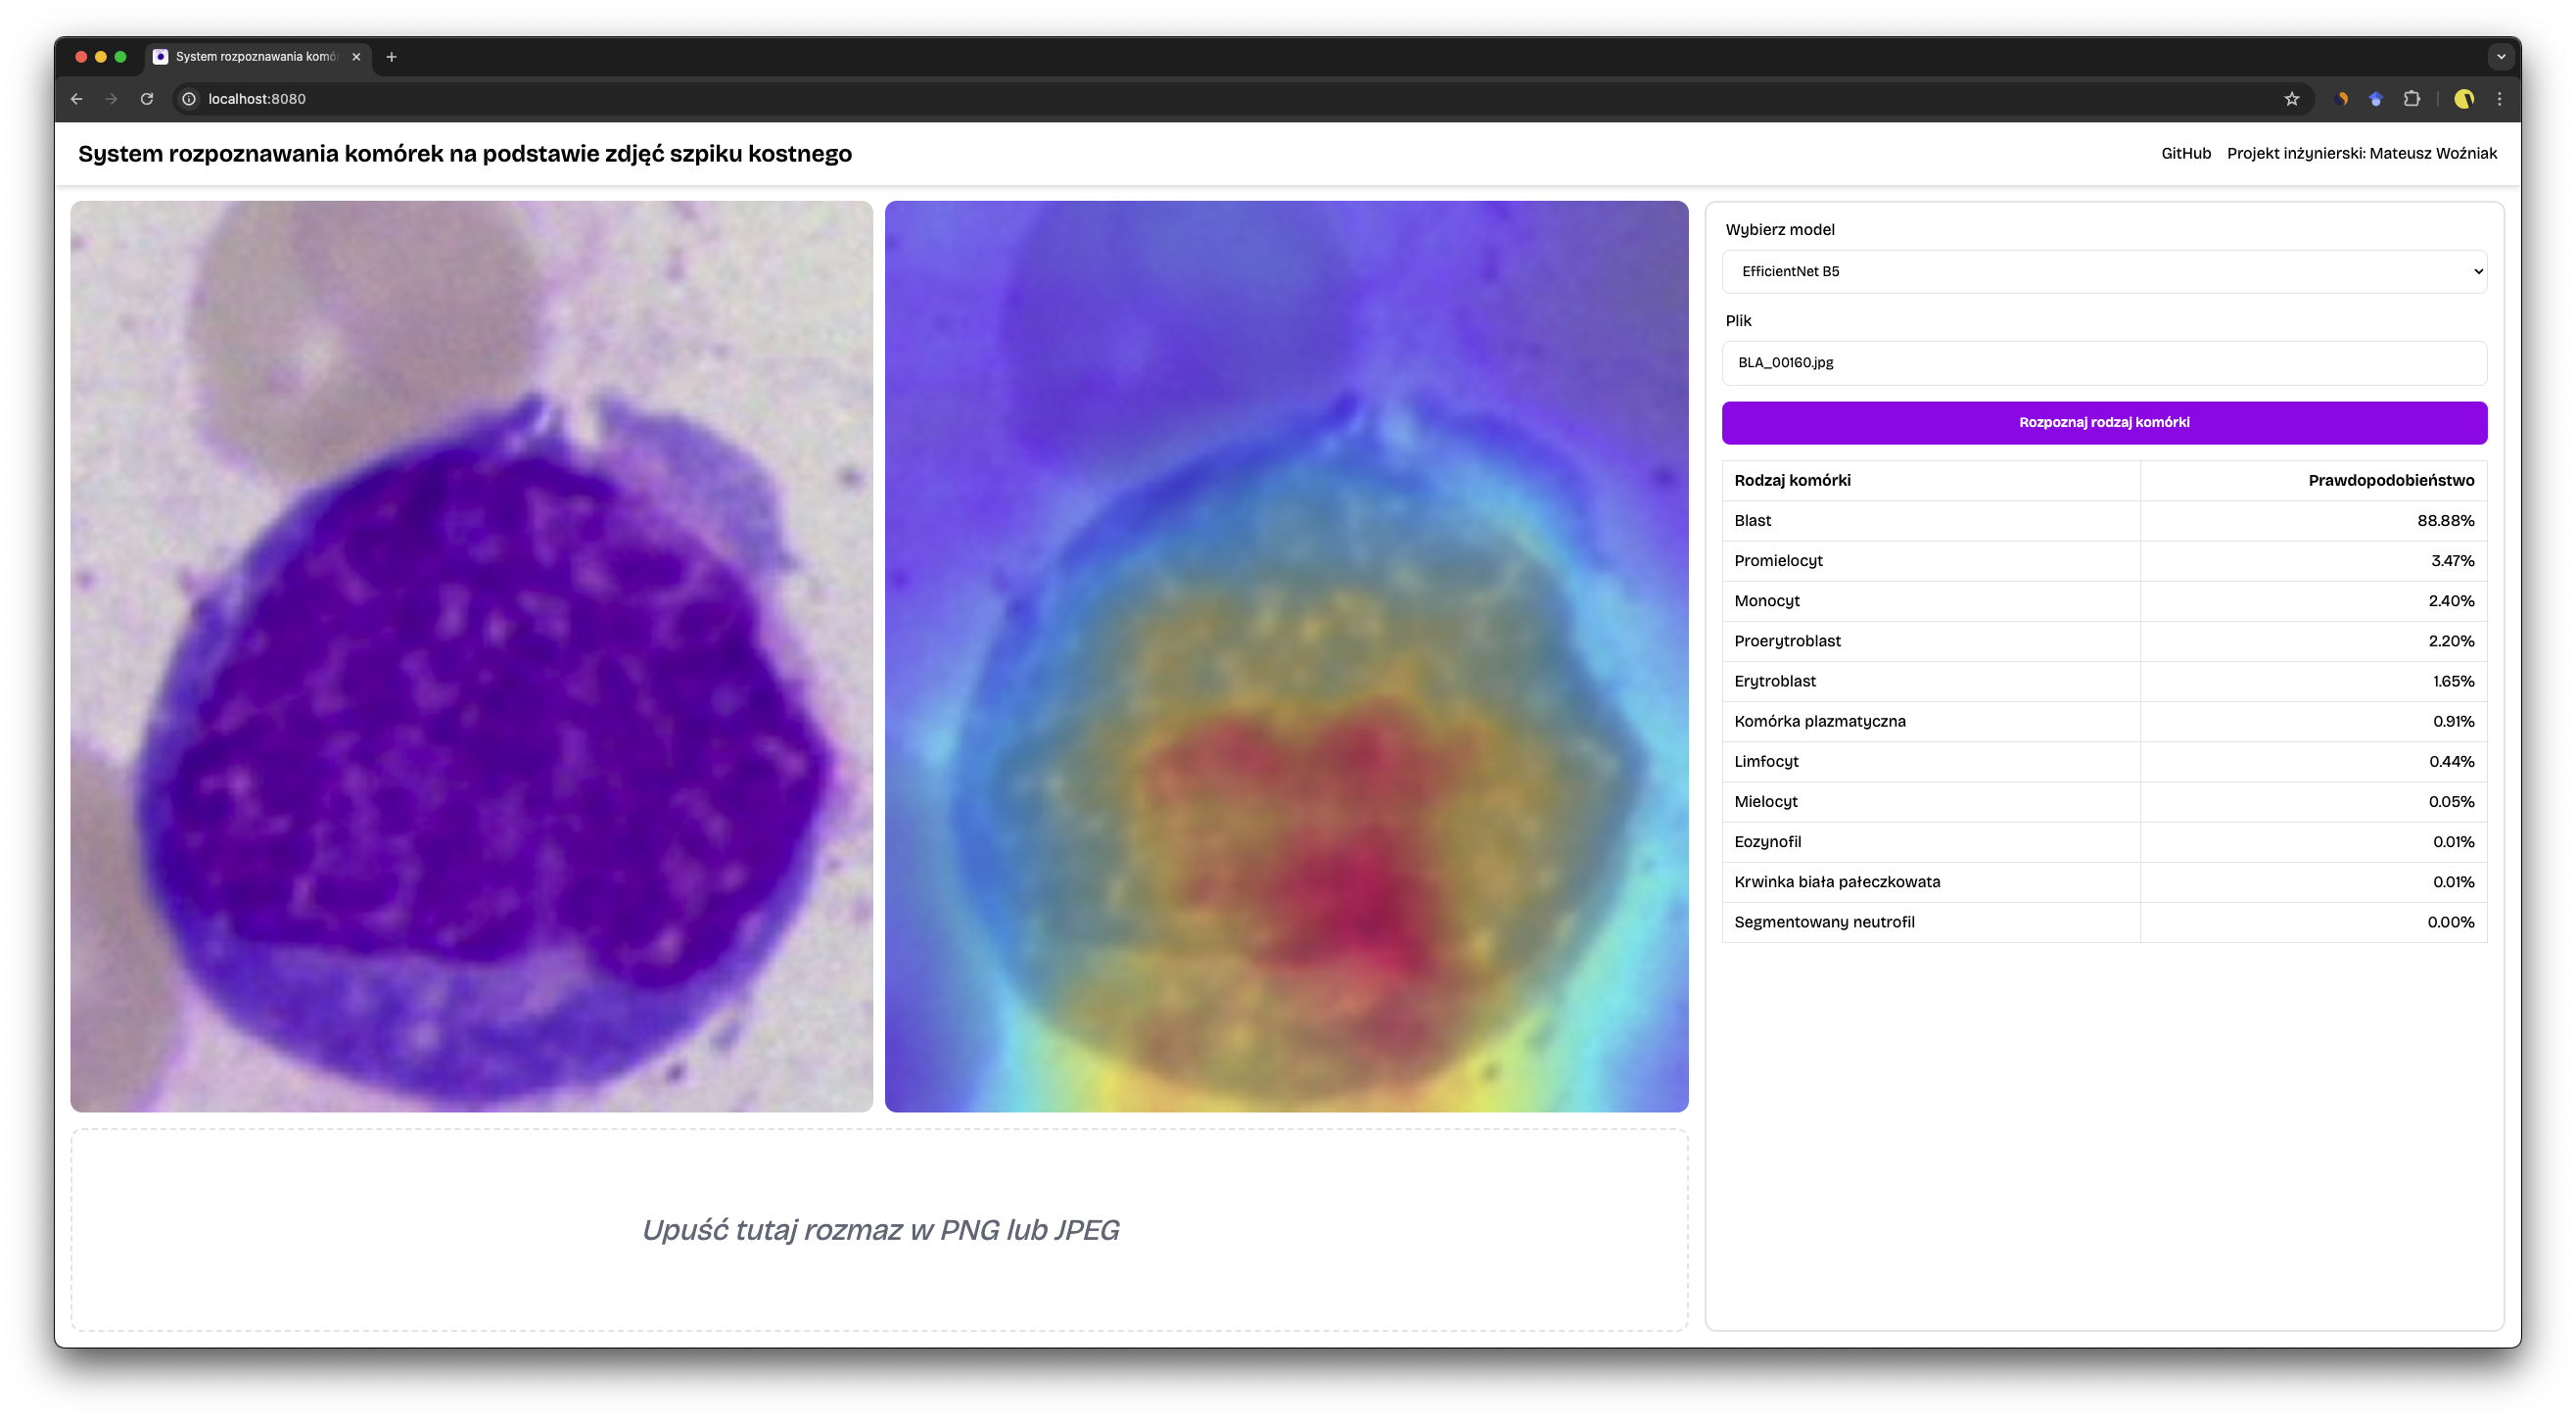
\includegraphics[width=\textwidth]{app}
    \caption{Aplikacja internetowa do rozpoznawania komórek}
    \label{fig:ui}
\end{figure}


\begin{figure}
    \centering
    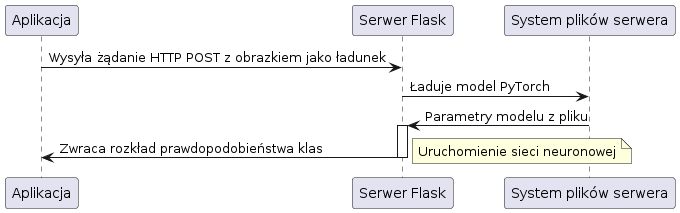
\includegraphics[width=0.8\textwidth]{arch}
    \caption{Architektura klient-serwer aplikacji internetowej i serwera Flask}
    \label{fig:arch}
\end{figure}

By skorzystać z aplikacji internetowej, należy przeciągnąć plik ze zdjęciem komórki do sekcji "Upuść tutaj rozmaz w PNG lub JPEG".
Po wysłaniu obrazu użytkownik może wybrać model i kliknąć przycisk "Rozpoznaj rodzaj komórki".
Następnie ukaże się tabela z rozkładem prawdopodobieństwa (po prawej stronie okna).
Stylizowanie aplikacji zostało wykonane z użyciem biblioteki CSS o nazwie \textit{Tailwind.css}~\cite{tailwind}.
Komunikacja klient-serwer jest zapewniona przez bibliotekę \textit{Axios}~\cite{axios}.
Architekturę przedstawia rys.~\ref{fig:arch}.


\section{Algorytm ekstrakcji obrazów komórek z dużego zdjęcia rozmazu}\label{sec:kwadraty}

Zbiór danych użyty w trakcie trenowania splotowej sieci neuronowej przedstawia komórki, które zajmują prawie całą cześć obrazu.
Innymi słowy, każdy obrazek stanowi wycinek dużego skanu z rozmazu.
Często jednak istnieje potrzeba zautomatyzowania procesu wycinania kwadratowych obrazów przedstawiających komórki z dużego skanu.
Zaproponowano algorytm korzystający z różnych metod wizji komputerowej do osiągnięcia tego zadania.

Niniejszy algorytm przyjmuje obraz przedstawiający kilkanaście komórek różnego rodzaju i eksportuje
każdą komórkę do kwadratowego zdjęcia.
Algorytm wykonuje następujące kroki w celu wyznaczenia komórek z obrazka:

\begin{figure}
    \centering
    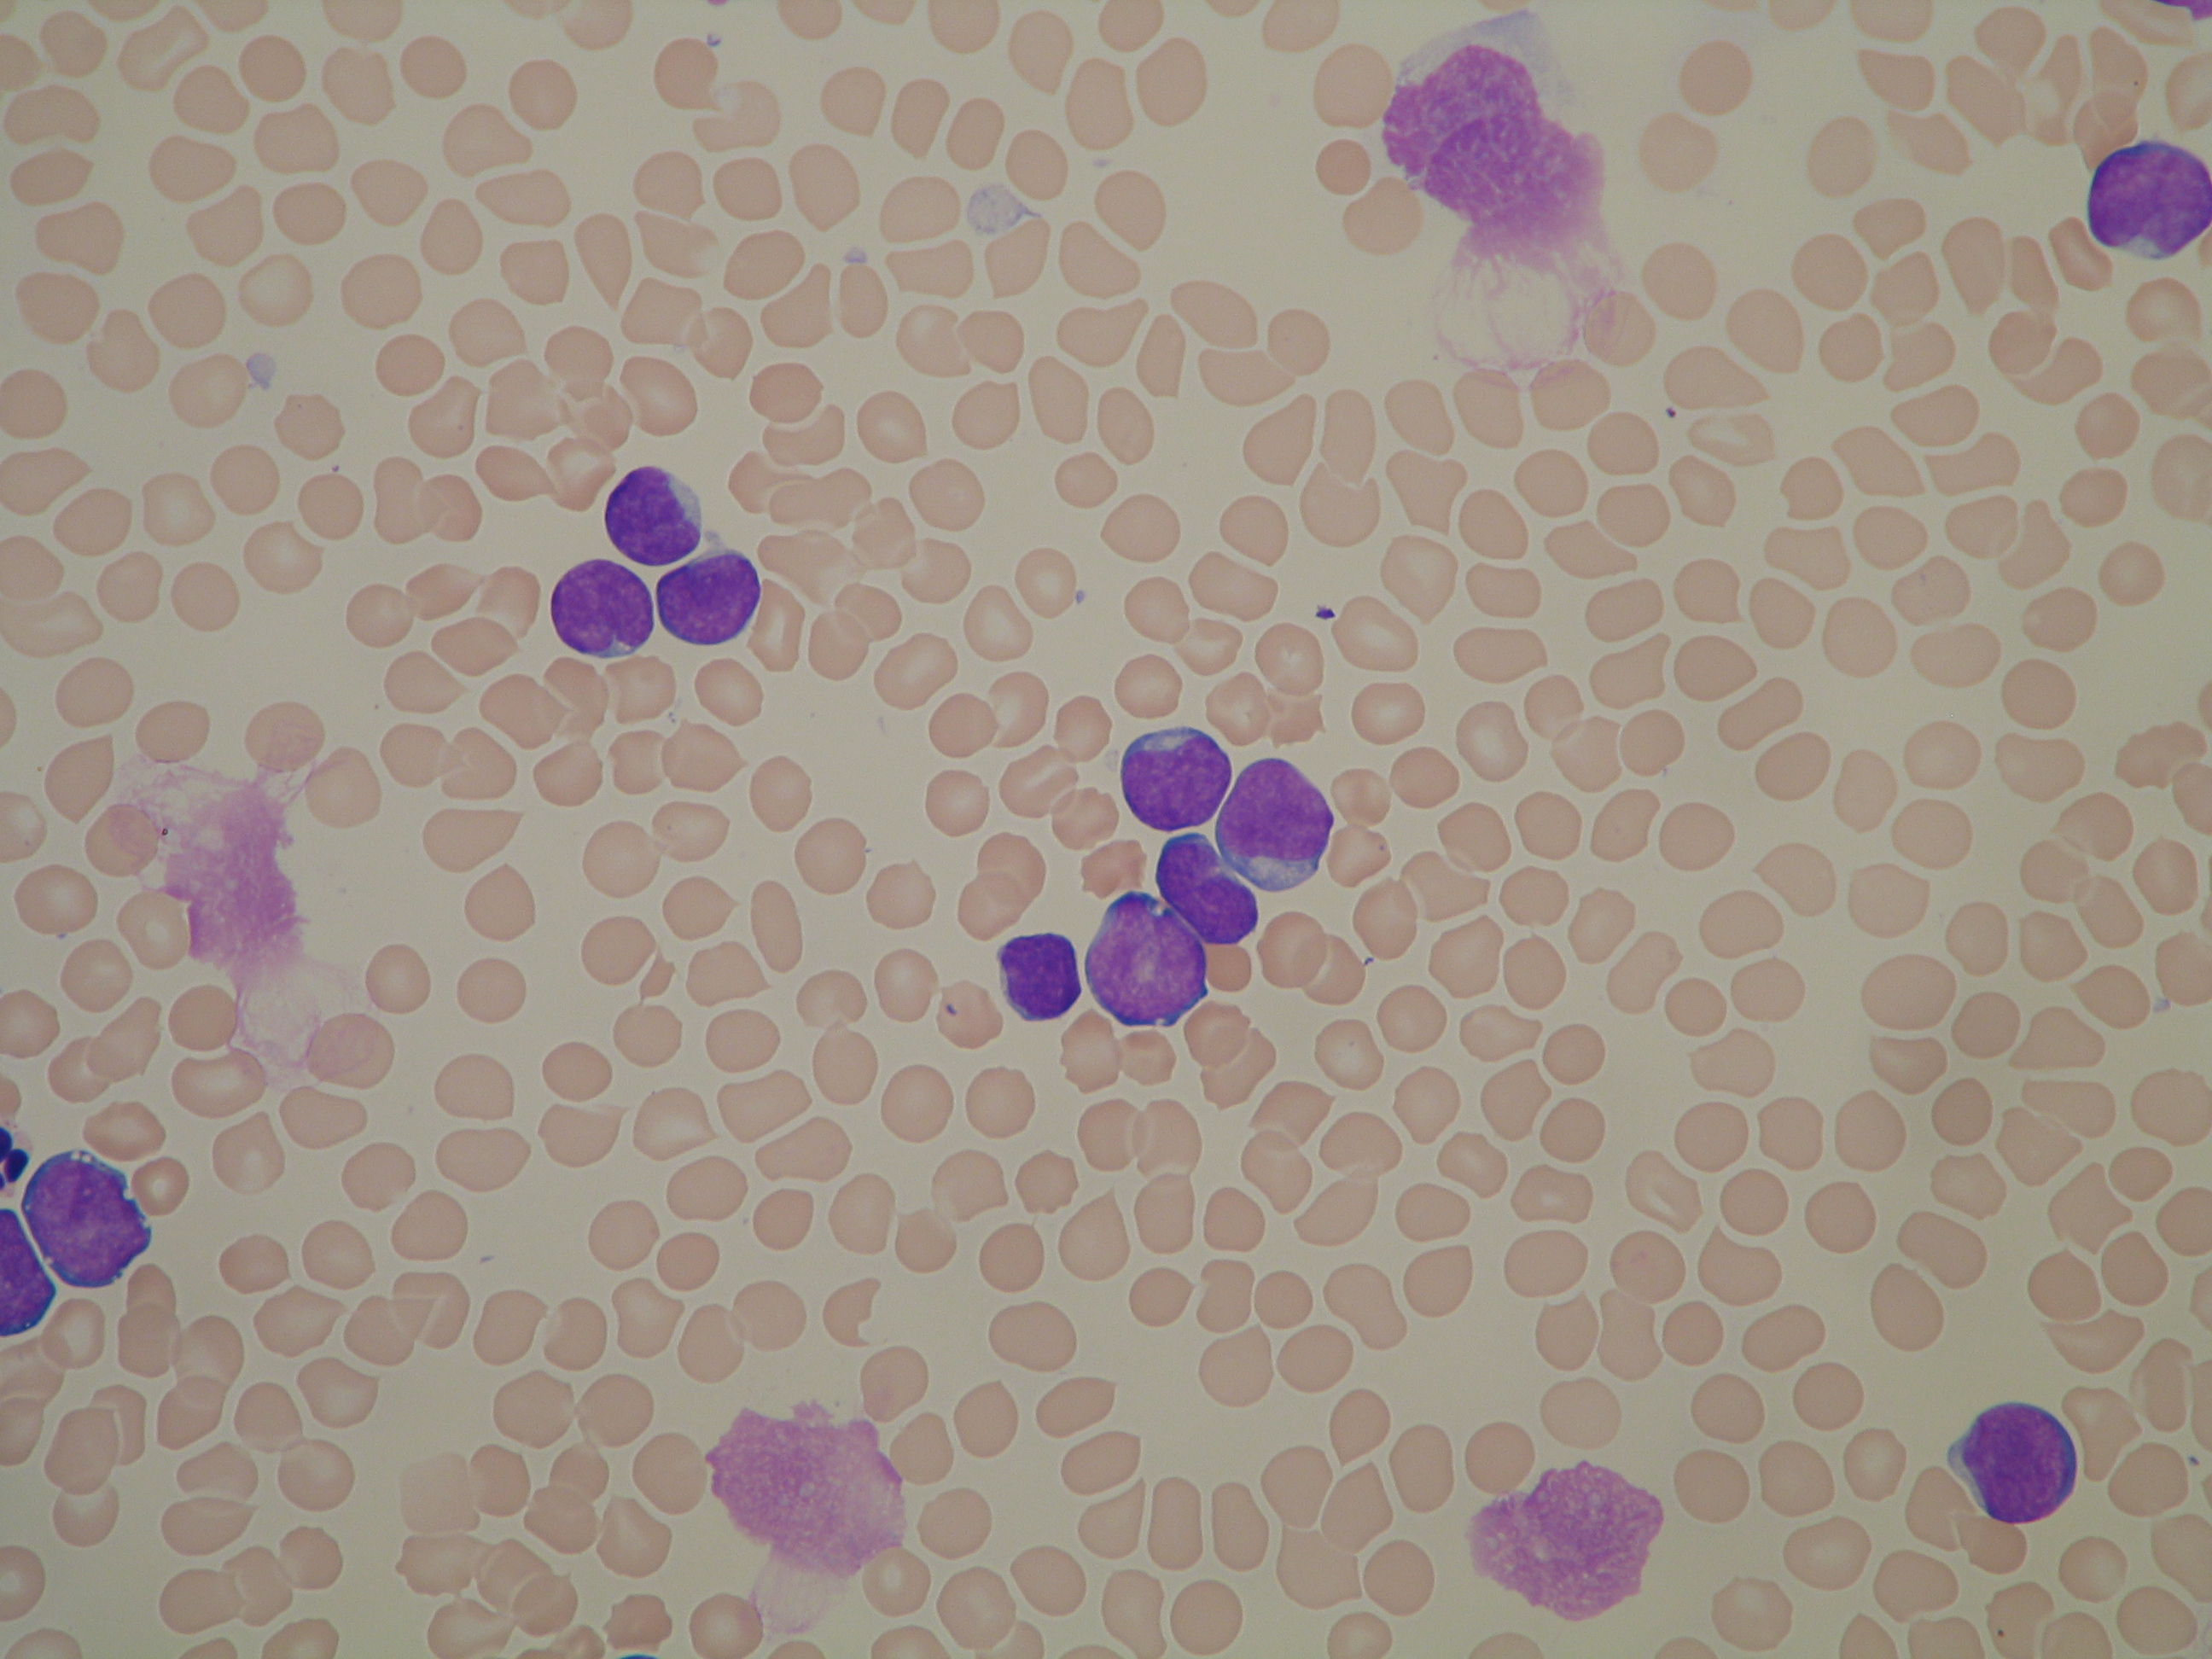
\includegraphics[width=0.8\textwidth]{Im060_1}
    \caption{Wejście algorytmu}
    \label{fig:extract_input}
\end{figure}

\begin{figure}
    \centering
    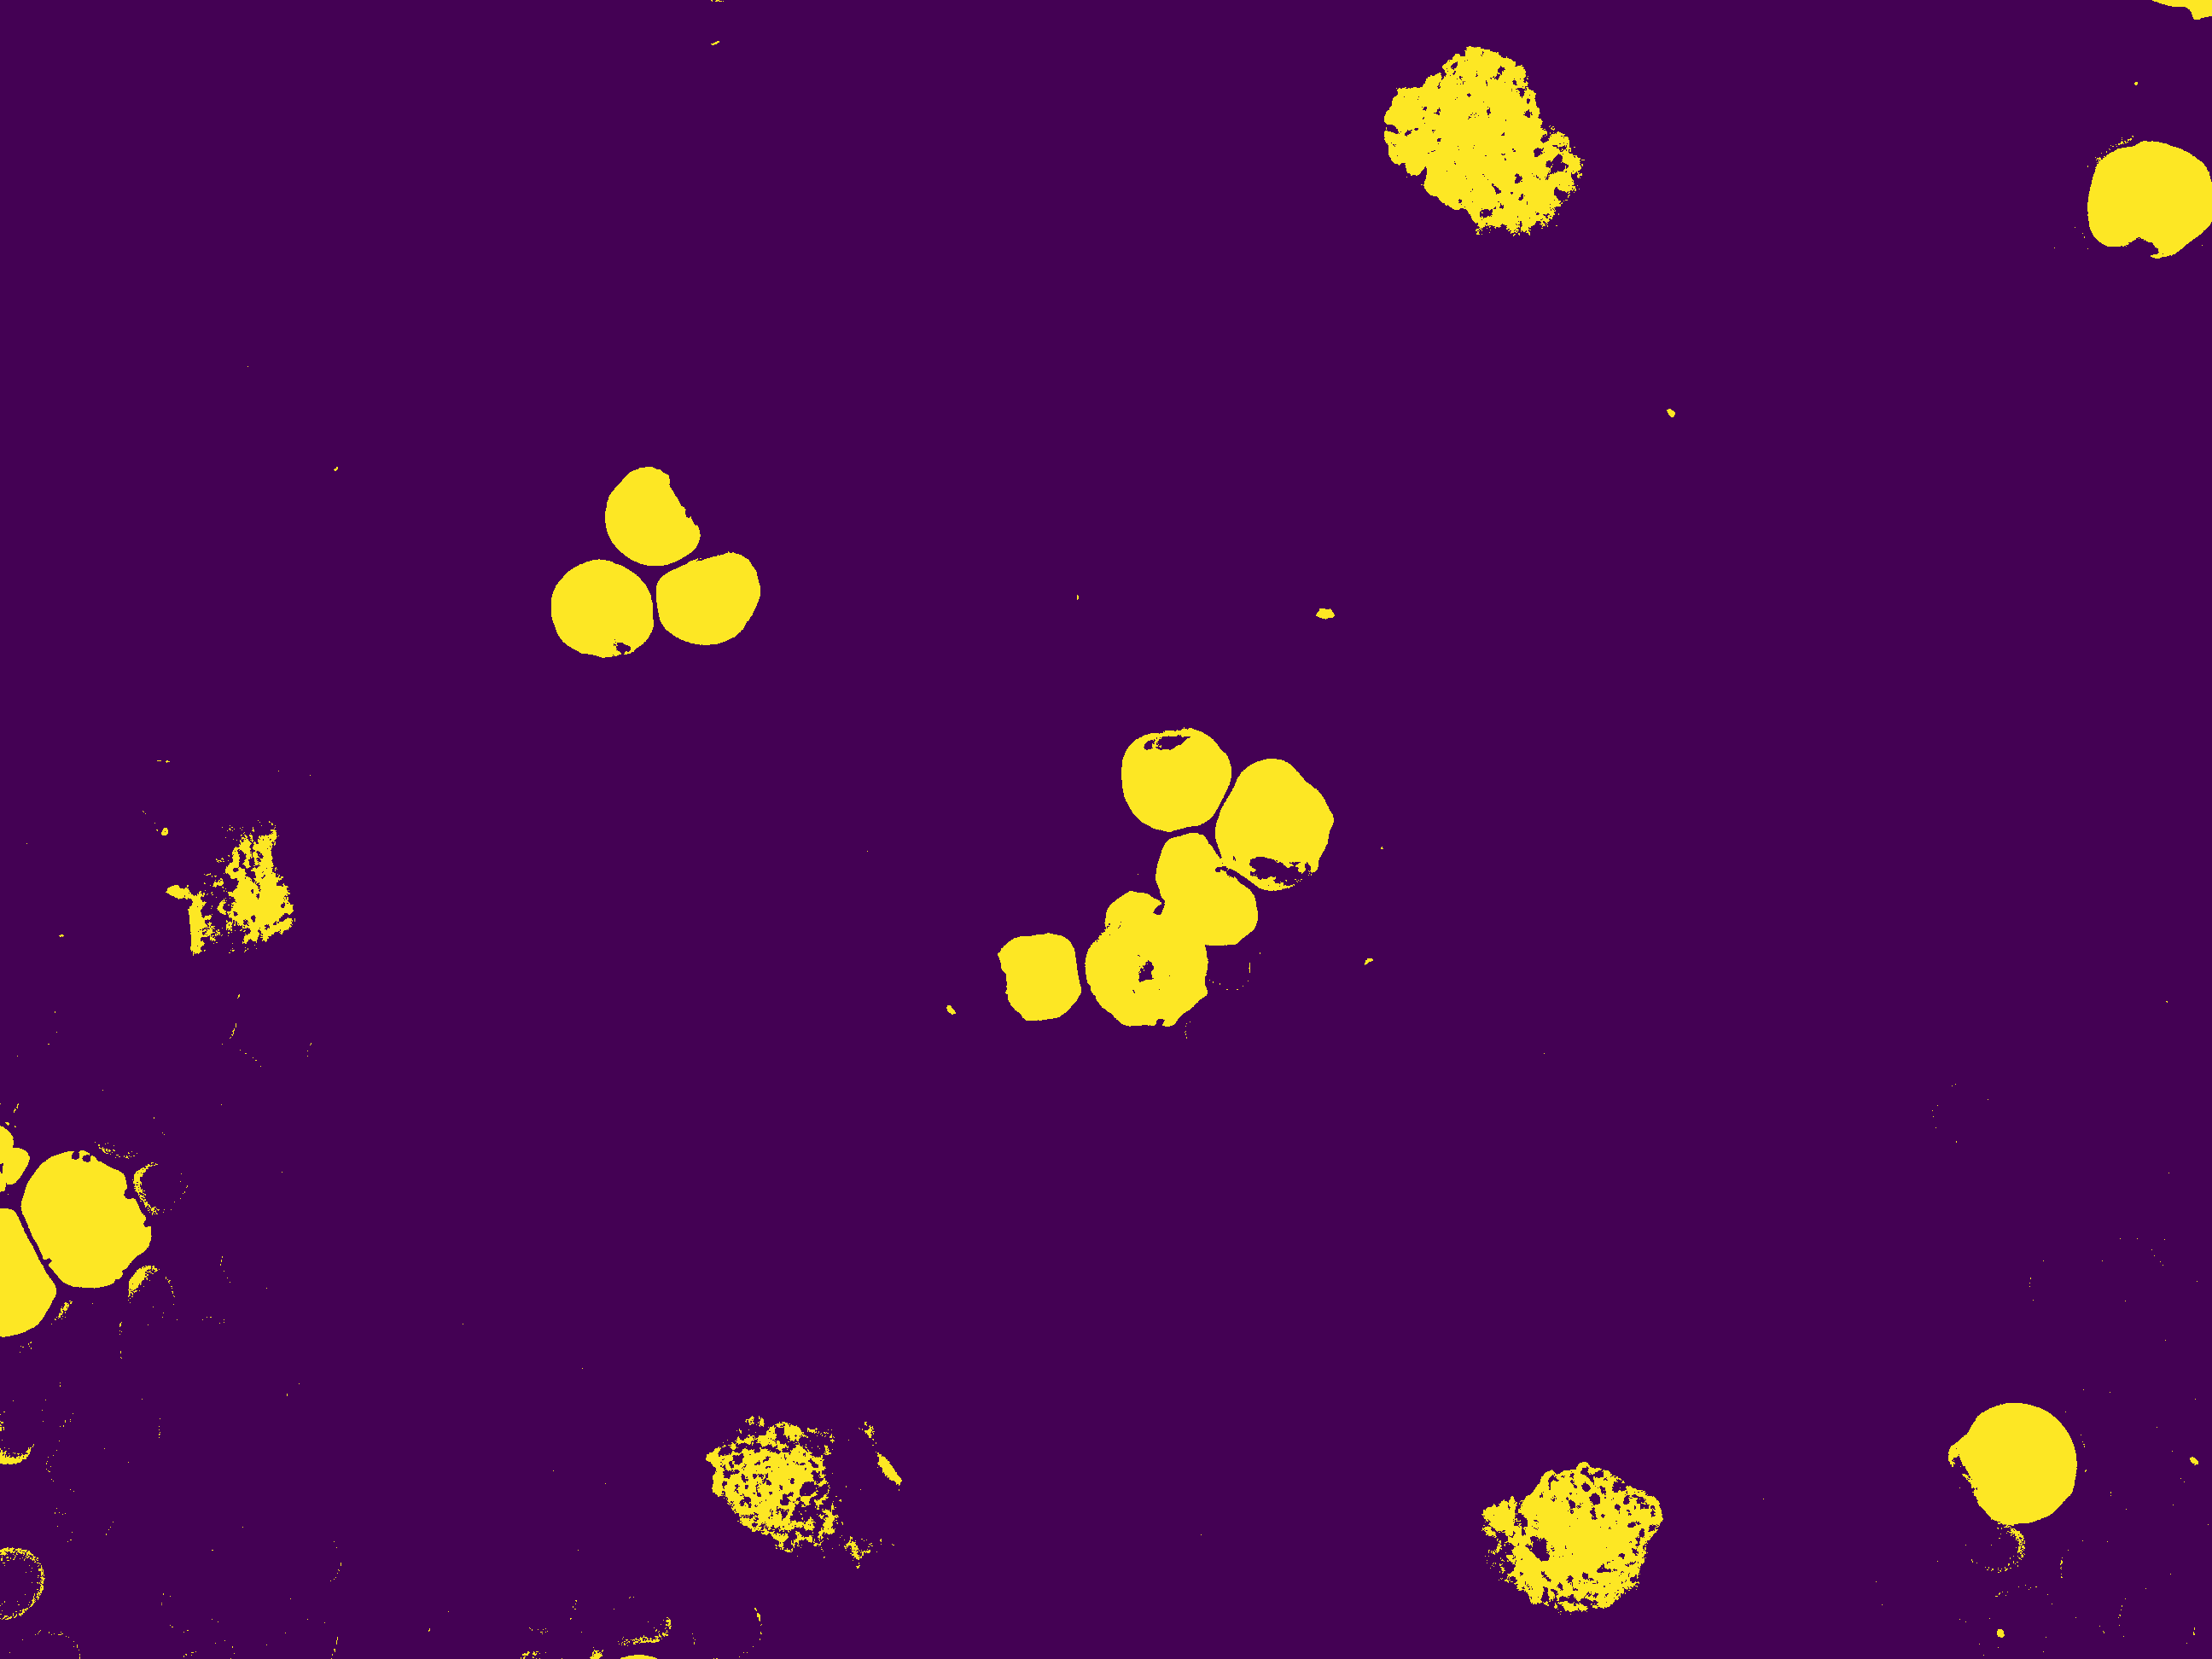
\includegraphics[width=0.8\textwidth]{Im060_1_thresh}
    \caption{Obrazek po progowaniu}
    \label{fig:extract_thresh}
\end{figure}

\begin{figure}
    \centering
    \includegraphics[width=0.8\textwidth]{Im060_1_contours}
    \caption{Oznaczone kontury wraz z punktami centralnymi}
    \label{fig:extract_contours}
\end{figure}

\begin{figure}
    \centering
    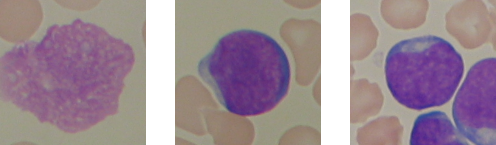
\includegraphics[width=0.8\textwidth]{cells}
    \caption{Wyekstraktowane kwadratowe obrazki}
    \label{fig:extract_squares}
\end{figure}

\begin{enumerate}
    \item Konwersja oryginalnego obrazu (rys.~\ref{fig:extract_input}) na skalę szarości.
    Jest to konieczne, ponieważ progowanie w kroku drugim nie może odbywać się na obrazie kolorowym.
    Do konwersji zastosowano funkcję \textit{cv2.cvtColor} - pozwala ona konwertować obraz z jednej przestrzeni kolorów do innej.
    \item Progowanie z pomocą algorytmu Otsu~\cite{otsu}.
    Jest to algorytm adaptacyjnego progowania, często stosowany do analizy obrazów medycznych.
    Progowanie ma na celu wyodrębnienie ciemniejszych obszarów obrazu - cytoplazmy i jądra komórek (rys.~\ref{fig:extract_thresh}). Otsu jest algorytmem progowania globalnego i opiera się na analizie histogramu.
    Dąży on do maksymalizacji wariancji międzyklasowej.
    \item Wyznaczenie konturów z pomocą funkcji \textit{cv2.findContours}~\cite{contours}.
    Kontur jest definiowany jako pewna ciągła krzywa, która łączy punkty o tej samej intensywności.
    W opisanym algorytmie kontury mają za zadanie informować o granicach komórki.
    Argumentem funkcji jest flaga \textit{cv2.RETR\_EXTERNAL}, która powoduje, że zwrócone zostają jedynie najbardziej zewnętrzne kontury - kontury wewnętrzne są ignorowane.
    \item Obliczanie punktów centralnych konturów za pomocą momentów Hu. Każdy wyznaczony punkt centralny jest traktowany jako środek komórki (rys.~\ref{fig:extract_contours}).
    Współrzędne punktów centralnych można wyznaczyć na podstawie momentów Hu, korzystając ze wzorów~\ref{eq:hu_x} i~\ref{eq:hu_y}.
    \begin{equation}
        \bar{x} = \dfrac{M_{10}}{M_{00}}\label{eq:hu_x}
    \end{equation}
    \begin{equation}
        \bar{y} = \dfrac{M_{01}}{M_{00}}\label{eq:hu_y}
    \end{equation}
    \item Wycięcie obszaru komórki za pomocą indeksów Python (rys.~\ref{fig:extract_squares}). Obraz każdej znalezionej komórki trafia do osobnego pliku w folderze wyjściowym.
    Do zapisu na dysk wykorzystano funkcję \textit{matplotlib.pyplot.imsave()}.
\end{enumerate}

Kod opisanego algorytmu przedstawia listing~\ref{lst:extract}.

\lstinputlisting[label={lst:extract}, caption={Kod wycinający obraz komórki z dużego skanu mikroskopowego}, language=ipython]{extract.py}